
\chapter{Results and Discussion}
\label{chap:results_and_discussion}

\section{Experimental Results}
\label{sec:experimental_results}

Using the indoor motion platform described in Section \ref{sec:development_of_linear_motion_platform} and the experimental setup described in Section \ref{sec:scene_design}, images from three individual scenes with depths ranging up to \nicetilde0.4m were captured.
The motion platform velocity was controlled and was measured at $v_c = 0.021m/s$, the Lytro exposure time was varied from 1/6.4s to 1/2s and the Lytro ISO setting set to automatic to maintain scene brightness.

The Lytro depth maps were calibrated using the shallow depth range mapping described in Figure \ref{fig:depth_real_world_vs_lytro_response}.
The depth map data was then used to de-blur the light fields, using the technique described in Section \ref{sec:image_processing_and_deconvolution}.
For comparison, the light field images were also de-blurred using the Richardson-Lucy method, blind deconvolution and a simple regularized deconvolution implementation, all with a single PSF computed at the median scene depth.

The computed Q-factors and estimated RMSE noise levels are shown in Tables \ref{tab:deblurred_light_field_q_factors} and \ref{tab:deblurred_light_field_rmse_estimates}.


\begin{table}[h]
\centering
\caption[De-blurred light field Q Factors]{De-blurred light field Q Factors (larger indicates more high-frequency content)}
\label{tab:deblurred_light_field_q_factors}
\begin{tabular}[h]{r | c c c}
                & Milo & House & Bears \\
\hline
Original        & 1.00 & 1.00  & 1.00 \\
Ours            & 2.26 & 1.56  & 1.68 \\
Blind           & 1.60 & 1.92  & 1.69 \\
Regularised     & 2.23 & 2.68  & 2.53 \\
Richardson-Lucy & 1.62 & 1.93  & 1.69 \\
\end{tabular}
\end{table}


\begin{table}[h]
\centering
\caption[De-blurred light field RMSE Estimates]{De-blurred light field RMSE Estimates (smaller indicates less image noise)}
\label{tab:deblurred_light_field_rmse_estimates}
\begin{tabular}[h]{r | c c c}
                & Milo  & House & Bears \\
\hline
Original        & 3.96  & 2.72 & 3.18 \\
Ours            & 5.90  & 3.94 & 4.15 \\
Blind           & 9.06  & 4.98 & 4.14 \\
Regularised     & 11.23 & 7.22 & 5.78 \\
Richardson-Lucy & 9.19  & 4.99 & 4.15 \\
\end{tabular}
\end{table}


Selected light field images of the three scenes are shown in Figures \ref{fig:results_milo_long_b} to \ref{fig:results_bears_short}, along with the respective depth maps, our results, and results from 2D deconvolution.


\begin{figure}[h]
\centering
\includegraphics[width=\textwidth]{results_milo_long_b.pdf}
\caption[De-blurring results - \enquote*{Milo} Scene]{
De-blurring results - \enquote*{Milo} Scene.
ISO Setting: 75, Exposure time: 1/2s.
a) Original blurred scene b) Lytro depth map normalised for display c) Our de-blurred result, and results from 2D blind (d), regularised (e) and Richardson-Lucy (f) deconvolution.
Note that in (c) the text on the ground is sharp at all scene depths.
}
\label{fig:results_milo_long_b}
\end{figure}

\begin{figure}[h]
\centering
\includegraphics[width=\textwidth]{results_house_short.pdf}
\caption[De-blurring results - \enquote*{House} Scene]{
De-blurring results - \enquote*{House} Scene.
ISO Setting: 207, Exposure time: 1/6.4s.
a) Original blurred scene b) Lytro depth map normalised for display c) Our de-blurred result, and results from 2D blind (d), regularised (e) and Richardson-Lucy (f) deconvolution.
Note the ringing in the background is more pronounced in (d)-(f) than in our de-blurred image (c).
}
\label{fig:results_house_short}
\end{figure}

\begin{figure}[h]
\centering
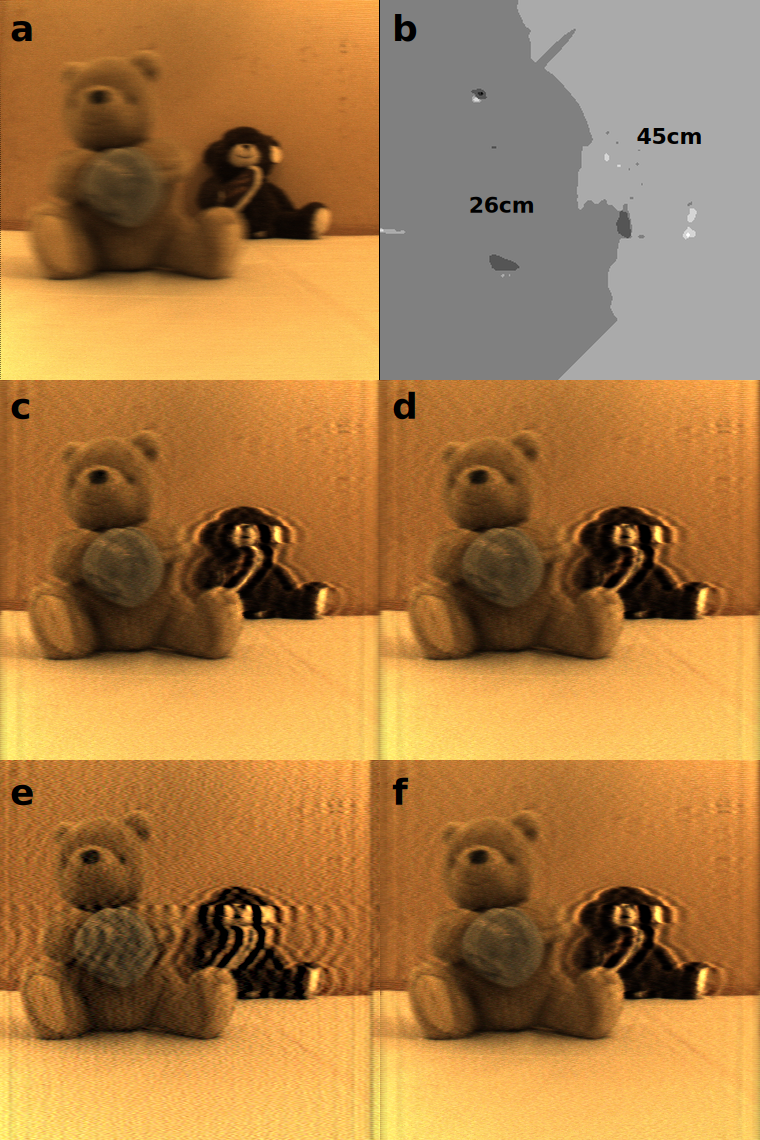
\includegraphics[width=\textwidth]{results_bears_short.pdf}
\caption[De-blurring results - \enquote*{Bears} Scene]{
De-blurring results - \enquote*{Bears} Scene.
ISO Setting: 113, Exposure time: 1/2s.
a) Original blurred scene b) Lytro depth map normalised for display c) Our de-blurred result, and results from 2D blind (d), regularised (e) and Richardson-Lucy (f) deconvolution.
In these results there is little difference between images (c) and (d-f) due to the lack of significant scene depth change, and the poor quality depth map.
}
\label{fig:results_bears_short}
\end{figure}



\section{Discussion}
\label{sec:discussion}

Table \ref{tab:deblurred_light_field_q_factors} shows that the Q factor increased for each test scene using our de-blurring method.
Additionally, the Q-factors from the 2D deconvolution methods increased for each scene.
This indicated that after de-blurring, the light field images contained a greater proportion of high-frequency content in the horizontal direction.
This can be seen visually in the de-blurred light field images.
Note that, as stated in section \ref{sec:quantitative_analysis}, the Q-factor does not discriminate between high-frequency content due to a lack of motion smear and high-frequency content due to false ringing edges created by noise amplification.
This is highlighted for example in Figure \ref{fig:results_milo_long_b}e, where a Q-factor of 2.23 was observed, yet the image is completely corrupted by ringing artifacts, instead of being a sharp image of the ground truth scene.

For this reason the RMSE noise estimate was used as a second quantitative metric.
The RMSE noise figures in Table \ref{tab:deblurred_light_field_rmse_estimates} indicate that our de-blurring method raised the RMSE noise less than the 2D deconvolution methods for the \enquote*{Milo} and \enquote*{House} scenes, and raised the RMSE noise level by a comparable amount for the \enquote*{Bears} scene.
The RMSE values for the regularised de-blurring method are larger than those for all other methods, reflecting the more visible presence of ringing in Figures \ref{fig:results_milo_long_b}e, \ref{fig:results_house_short}e and \ref{fig:results_bears_short}e.
Our de-blurring method's RMSE noise performance in the \enquote*{Bears} scene was comparable to that of the 2D deconvolution methods due to the lack of significant depth difference in the scene, and the low quality depth map present for that scene.
The poor quality depth map was in this case caused by a lack of scene structure in all parts of the scene.
As stated in section \ref{sec:experimental_results}, the 2D deconvolution methods used a single PSF computed from Equation \ref{eq:blur_width_simple} using the median scene depth.
Thus, for the \enquote*{Bears} scene, the PSF used for the 2D deconvolution methods was similar in width to the PSFs used by our method, the result being that our method showed only slightly better or equal performance when compared with 2D deconvolution methods.

Figure \ref{fig:results_milo_long_b} most clearly shows the benefit of our method over 2D deconvolution methods; for example the text on the ground is de-blurred continuously though all scene depths, a feat which is impossible for 2D deconvolution methods to do.

In Figure \ref{fig:results_house_short} the benefit of our method is less pronounced, however ringing in the background of the scene is more pronounced in the 2D deconvolution cases.
This reflects the fact that a single PSF was used to de-blur a scene with varying degrees of motion blur.
In this case, the PSF used was sub-optimal for the degree of motion blur present in the background, and thus introduced excess ringing.

Figure \ref{fig:results_bears_short} again shows little difference between our method and the 2D deconvolution methods.
In this case, as explained above, this is due to the presence of only two major depth planes in the scene and the poor quality depth map.
Looking closely at the background bear's face reveals sharper features in our result than in the other cases.

\section{Implications}
\label{sec:implications}

By analysing the projective geometry camera equation (Equation \ref{eq:camera_projection}), we have shown that real-world depth measurements can be combined with knowledge of a camera trajectory and camera intrinsics to compute 3D point-spread functions.
This was verified experimentally, as shown in Figure \ref{fig:blur_vs_depth}.
We suggest that a 3D PSF is better than a 2D PSF as it allows for depth-aware deconvolution.
This type of deconvolution allows an optimal PSF to be used for all parts of an image, reducing ringing artifacts and increasing the quality of the de-blurred image.
For a practical demonstration of depth-aware deconvolution, we investigated the possibility of de-blurring light field images from a commercial Lytro camera.

Our initial experimental work suggested that Lytro depth maps are consistent for light field images with similar overall depth range.
This implies that if a rough estimate of the scene depth can be made, Lytro depth maps can be calibrated using a piecewise linear mapping.
We suggest that user-supplied scene information (e.g. from the \enquote*{scene} setting on a commercial camera), a cheap depth sensor such as an IR or ultrasound based focal-range sensor or \emph{a-priori} knowledge of a robotic operating environment can be used to this end.

The experimental results of our de-blurring tests show that linearly motion-blurred light field images from a Lytro camera can be de-blurred at all scene depths.
In order to do this, a rough estimate of the scene depth range is needed to calibrate the Lytro depth data, and the camera velocity, exposure time and focal length need to be known.
This technique however is not limited to Lytro images.
Our depth-aware deconvolution method could also be applied to images from any RGBD sensor that can provide calibrated depth maps, e.g. the Microsoft Kinect sensor. 
Using the Lytro camera is beneficial in this regard as de-blurred light field data can be obtained, opening more possibilities for computational photography.

Future practical applications of depth aware deconvolution include improving consumer satisfaction with hand-held light field and RGBD camera devices by de-blurring camera shake.
This will be more widely applicable in the near future, given that consumer smartphones are beginning to be equipped with depth-sensing capabilities \cite{google2014lensblur, google2014tango}.

Depth-aware deconvolution also has potential benefits for forensic and photo-restoration applications, even where depth information is not readily available.
For example the specification of a depth map could potentially be performed through interactive user input with one or more images \cite{sinha2008interactive}.
By exploiting user supplied \emph{a-priori} information about the content of a photo in this way, it may be possible to perform depth-aware deconvolution even on photos where a depth map is not available. 

Finally, we anticipate that depth-aware deconvolution will have benefits in robotic navigation and computer vision applications.
Robotic systems have many attributes that make them suitable for depth-aware deconvolution; often camera intrinsics are known, and the exposure time of images can be obtained, camera trajectory will likely be known thanks to motion encoders or other robotic sensors, and increasingly, more robotic systems are incorporating highly capable depth sensors.
Light field sensors such as the Lytro have the potential to be powerful tools for robotic systems, and by demonstrating the ability to de-blur a light field image, it is hoped that the performance of robotic light field computer vision systems can be improved, e.g. in low-light operating environments where motion blur is more likely.


\section{Limitations and Future Work}
\label{sec:limitations_and_future_work}

The work presented here has several limitations relating to the experimental method, the volume of data used and the types of light field images tested.

Our de-blurring method was demonstrated with linear motion blur only.
Equation \ref{eq:camera_projection} can equally be applied to compute a 3D PSF for optical-axis rotational camera motion, or even generalized camera trajectories.
Future work could explore if these PSFs can be used in the same way for de-blurring.

In the experiments performed the camera velocity used to compute the PSF was supplied \emph{a-priori}.
In a robotic system this information could potentially come from encoders, an inertial measurement unit or other velocity sensors.
Additionally, using calibrated depth data, future work could explore the possibility of using blind deconvolution methods to simultaneously recover the real-world camera velocity \emph{and} high-frequency image details.

The images used for in these experiments were all captured in a controlled environment.
Real-world implementations of this de-blurring method would need to be tested for robustness against lighting and other scene variations.

Light field pixel confidence maps are available in the Light Field Toolbox, and the Lytro desktop software supplies depth confidence maps along with the depth data.
Neither of these sources of information were utilised in the experiments performed here.
Future work could look at integrating this data into the de-blurring process, perhaps as a means for suppressing noisy regions of the light field, or regions where there is little confidence in the light field depth map.

Although many light field images were captured and analysed in the process of developing the light field de-blurring technique, only three scenes were used for the final analysis.
Future work could look at confirming the results found in this experiment by collecting more data.

The Lytro camera was the only light field camera used in this experiment.
The Lytro generates a light field with a specific dimensionality; for example Lytro light field images have a much larger spatial resolution than angular.
Future work could explore the use of other light field cameras, or more generally, light fields with other shapes (e.g. more angular resolution).

At this point, the light field de-blurring is necessarily an off-line process, as the Lytro desktop companion software must be used to download light field images before they can be processed.
Future work could look into reverse-engineering the Lytro camera USB or Wifi download protocols, allowing Lytro cameras to be integrated on-line into mobile robotic systems. 

Additionally, the de-blurring implementation shown here is computationally intensive, and no effort has been made to optimise the process.
Before this work could be implemented in any real world system, robotic or otherwise, the de-blurring process would need to be optimised to run much more efficiently.

For simplicity these experiments focused only on global motion blur caused by camera motion.
Future work could look into individual object blur, and applications for selectively de-blurring isolated objects in a scene.

As shown in section \ref{sec:light_field_depth_estimation}, the presence of motion blur reduces the quality of the light field depth estimation, which is required for de-blurring.
This fact suggests several possibilities for future work; techniques for more robust, blur-invariant light field depth estimation are needed.
Alternately, the method presented here could potentially be adapted to an iterative form, where an initial de-blurring pass allows better depth estimation, followed by another de-blurring pass etc.

Finally, insufficient data was collected to fully quantify the Lytro depth map response function.
Further research with ground truth depth data is needed to better understand the limitations and behavior of the Lytro depth maps, especially in uncontrolled real-world scenes.

